\documentclass{article}
\usepackage{amsfonts}
\usepackage{graphics}
\setlength{\textwidth}{17cm}
\setlength{\textheight}{9in}
\setlength{\topmargin}{-1.5cm}
\setlength{\oddsidemargin}{0in}
\setlength{\evensidemargin}{0in}
\newcommand{\unw}{ {\cal K}}
\newcommand{\sbody}[2]{ {\textstyle {#1 \over #2} } }
\newcommand{\Q}{\mathbb{Q}}
\newcommand{\R}{\mathbb{R}}
\newcommand{\C}{\mathbb{C}}
\newcommand{\Z}{\mathbb{Z}}
\newcommand{\sgn}{ \mathop {\rm sgn}\nolimits}
\newcommand{\Sin}{ \mathop {\rm Sin}\nolimits}
\newcommand{\Arcsin}{ \mathop {\rm Arcsin}\nolimits}
\newcommand{\Arctan}{ \mathop {\rm Arctan}\nolimits}
\newcommand{\invsin}{ \mathop {\rm invsin}\nolimits}
\newcommand{\invsh}{ \mathop {\rm invsh}\nolimits}
\newcommand{\invcos}{ \mathop \mathrm{invcos} \nolimits}
\newcommand{\invtan}{ \mathop \mathrm{invtan} \nolimits}
\newcommand{\asin}{ \mathop {\rm asin}\nolimits}
\newcommand{\acos}{ \mathop {\rm acos}\nolimits}
\newlength{\funcwd}\newlength{\funcht}
\newcommand{\inverse}[1]{%  this macro is modelled on \face from the LaTeX book
\settowidth{\funcwd}{#1}\settoheight{\funcht}{#1}%
\raisebox{.9\funcht}{%
 \makebox[0pt][l]{\hspace{.1\funcwd}$\scriptstyle\vee$}}#1}
\newcommand{\inversef}[1]{% because f is italic, the v misses the top of the f otherwise
\settowidth{\funcwd}{#1}\settoheight{\funcht}{#1}%
\raisebox{.9\funcht}{%
 \makebox[0pt][l]{\hspace{.5\funcwd}$\scriptstyle\vee$}}#1}

\begin{document}

\title{The multi-valued nature of inverse functions}
\author{D.J.Jeffrey\\
Department of Applied Mathematics\\
University of Western Ontario\\
\texttt{djeffrey@uwo.ca}}
\date{Working Draft, September 2001}
\maketitle

\abstract{
A new treatment is given of the elementary inverse functions.
The new approach addresses the difference between the single-valued inverse function
defined by computer systems and the multi-valued function which represents the multiple
solutions of the defining equation.
The approach takes an idea from complex analysis, namely the \textit{branch} of an inverse
function, and defines an index for each branch.
The branch index then becomes an additional argument to the (new) function.
A benefit of the new approach is that it helps with
the general problem of correctly simplifying expressions containing inverse functions, which
has always been difficult both for humans and for computer algebra systems.
The new approach also can be extended to non-elementary inverse functions such as the
Lambert W function, which otherwise cannot be handled.
The difference between this approach and that of Riemann surfaces lies in the fact that
Riemann surfaces distinguish between branches by dividing the \textit{domain} of the
function into sheets, whereas here the range of the function is indexed.
}

\section{Introduction}
Two developments in mathematics suggest the need for a new treatment of multi-valued
functions, including the elementary inverse functions.
The developments are, first, the implementation of inverse functions in
computer-based mathematical systems and, second,
the appearance in the literature of new inverse functions.
The computer systems have struggled for years to find the best way to handle
possible simplifications such as
\begin{equation}\label{eq:Opening}
 (z^n)^{1/n}\, ?=\,?\, z\ ,\quad \arcsin(\sin z)\,?=\,?\,z\ , \quad \ln(e^z)\,?=\,?\, z\ ,
\end{equation}
as indeed have mathematicians \cite{Corless:2000:AAS,unwind:1996}.
Numerical counter-examples are
\[ ((-1)^2)^{1/2}\ne -1\ ,\quad \arcsin(\sin 2\pi)\ne 2\pi\ ,
 \quad \ln(e^{3\pi i})\ne 3\pi i\ . \]
In the 1980s, mistakes like these could commonly be found in computer algebra
systems\footnote{Let's not point fingers at particular systems.}.
The new treatment offers one way of looking at such problems.
The other motivation is the study of the Lambert W \cite{LambertW:1996}
and other inverse functions, which have no trivial relation between their branches,
in contrast to the elementary inverse functions.

There are, in addition, \ae sthetic reasons.
Anyone who has taught inverse trigonometric functions, or the complex roots of a number,
knows how difficult students find the idea of multi-valued functions.
One of the reasons is that there is not really a single uniform treatment.
For example, every calculus textbook introduces inverse functions with a discussion of
multi-valuedness and then ignores it when justifying equations such as
\[ \int \frac{dx}{1+x^2} = \arctan x  \]
(Abramowitz \& Stegun \cite{AandS:1965} do this in the same chapter).
Of course there will always be different treatments of the subject, because of
the mathematical desire for a different point of view.
Mathematical topics are to mathematicians rather like antique vases are to
vase connoisseurs.
The connoisseurs are not content to look at their vases only from the front;
they want to pick them up and admire them from all angles.
In the same way, the mathematical pleasure of a topic is not exhausted by any single
treatment, however thorough.
Perhaps there is something of this in the present treatment, but it is argued
that there are practical reasons to change, and practical benefits to gain.

\section{A question of values}

The first question in any treatment of multi-valued functions
concerns their representation; the question can be dramatized as follows.
Does $\arctan(1)$ represent the single number $\pi/4$, or does it represent all the solutions
$x$ of the equation $\tan x=1$, as the set $\{ \pi/4+k\pi\, |\, k\in \Z \}$,
or does $\arctan(1)$ represent some quantity in between,
perhaps the single number $\pi/4+k\pi$ but with the value of $k$ being decided later?
One point of view was expressed by Carath\'eodory, in his highly regarded
book \cite{Cara:1958}.
Considering the logarithm function in the complex plane, he addressed the equation
\begin{equation}\label{eq:logmult3}
\ln z_1z_2=\ln z_1 +\ln z_2\ ,
\end{equation}
for complex $z_1,z_2$.
He commented \cite[pp.~259--260]{Cara:1958}:
\begin{quote}
The equation merely states that
the sum of one of the (infinitely many) logarithms of $z_1$ and one of
the (infinitely many) logarithms of $z_2$ can be found among the
(infinitely many) logarithms of $z_1z_2$, and conversely every
logarithm of $z_1z_2$ can be represented as a sum of this kind (with a
suitable choice of $\ln z_1$ and $\ln z_2$).
\end{quote}
In this statement, Carath\'eodory first sounds as though he thinks of $\ln z_1$
as a symbol standing for a set of values,
but then for the purposes of forming an equation he prefers to select one value from the set.
Whatever the exact mental image he had, the one point that is clear is that $\ln z_1$
does not have a unique value,
which is in strong contrast to every computer system.
Every computer system will accept a specific value for $z_1$
and return a unique $\ln z_1$.

Notice a further implication of equation (\ref{eq:logmult3}).
If $\ln z_1$ means a single value, then that value is no longer determined solely by the
value of $z_1$: the value to be given to $\ln z_1$ is also determined by the context.
For example, in the equation
\[ 3\ln(-1) = \ln[(-1)^3] =\ln(-1)\ ,\]
if the first $\ln(-1)$ obeys $\ln(-1)=i\pi$, then the last one must obey $\ln(-1)=3i\pi$.
It is completely impractical to require a computer system to analyze the context of
each function before evaluating it. This example uses the complex plane, but real-valued
examples can be given also.

The reference book edited by Abramowitz \& Stegun \cite[Chap 4]{AandS:1965} is another authoritative source,
and it can be used to provide a real-valued example.
It defines the solution of $\tan t=z$ to be $t=\Arctan z = \arctan z+k\pi$.
It then gives the equation
\[  \Arctan(z_1)+\Arctan(z_2) = \Arctan\frac{z_1+z_2}{1-z_1z_2} \ .\]
For $z_1=z_2=\sqrt3$, we have $\Arctan \sqrt3+\Arctan\sqrt3 =\Arctan(-\sqrt3)$.
This is satisfied if $\Arctan\sqrt3=\pi/3$, and $\Arctan(-\sqrt3)=2\pi/3$,
but that means we no longer have the relation $\Arctan(-z)=-\Arctan(z)$.
By comparing the Abramowitz \& Stegun definition with the statement of Carath\'eodory,
we can see that as far as equations are concerned, all authors favour an interpretation based on judiciously
selecting one value from the possible ones.

A completely different approach is taken by Adams \cite{Adams:1999:SVC}.
He makes the inverse functions single valued by restricting the domain of the
defining function. Thus he defines
\[   \Sin x = \sin x\ , \mbox{only if} -\pi/2 \le x \le \pi/2\ .      \]
He then discusses the inverse of $\Sin x$, and not that of $\sin x$.
Thus in this approach there is
no doubt about the inverse function being unique, because $\Sin x=y$ has only one solution.
Since his book is a calculus textbook, the solution of $\sin x=y$ is not addressed.

In mathematical software, the interpretation of an inverse function as having a
single value is the best one.
Indeed it is the contention here that such an interpretation is always the best.
Further, the single value of a function should be determined by the
arguments to the function and not by the context in which it is placed.
All current computer systems return a single number when asked to evaluate,
at some specified point, a multi-valued function.
Therefore clearly for consistency any unevaluated symbolic quantity should also
represent a single value.

\section{The Lambert W function}
This function is an inverse function with properties that differ from the elementary
inverse functions.
It first received a name in the early 1980s, when \textsl{Maple}
defined a function that was named simply~$W$.
An historical search, conducted while writing an account of
this function~\cite{LambertW:1996}, found work by the eighteenth century
scientist J.~H.~Lambert that foreshadowed the definition of the function;
even though his work did not actually define the function, $W$ was
named in his honour.
The same search uncovered a fortuitous reason for calling the function~$W$,
in that E.~M.~Wright, a mathematician known for his book with Hardy on pure
mathematics, studied the complex values of the function, again without naming
it.

The definition of~$W$ is that it is the function that solves the equation
\begin{equation} \label{eq:MainDef}
W e^W =z\ ,
\end{equation}
where $z$ is a complex number.
This equation always has an infinite number of solutions, most of them complex.
There is always special interest in solutions that are purely real,
and so we note immediately that when
$z$ is a real number, equation (\ref{eq:MainDef}) has
no real solutions when $z<-1/e$; it has two real solutions when $-1/e<z<0$; and it has
one real solution when $z>0$.
Even if $z$ is real, there are still complex solutions.

A numerical example is $W e^W=-0.1$. The two real solutions are
$W=-0.1118326$, and $-3.577152$ as well as an infinite number of complex solutions,
the smallest of which are $W=-4.449098\pm 7.307061i$. The two real solutions were
labelled $W_p$ and $W_m$ by \cite{Barry:1995:RVW}; however, the labelling using an integer
introduced in \cite{LambertW:1996} is preferable, because it includes the complex case.

For present purposes, the important property $W$ has is the lack of a trivial relation
between the different values is takes for the same argument.

\section{The issues are complex}
The first multi-valued functions shown to mathematics students
are the inverse trigonometric functions,
because their multi-valued behaviour can be demonstrated using real numbers.
(The square root function is probably the very first, but the terminology
multi-valued is not deployed at that stage.)
This is in contrast to the logarithm function, whose multi-valued behaviour
appears only in the complex plane.
A treatment of multi-valued functions that extends easily into the complex plane, while
remaining comprehensible to those who work only on the real line is the target we aim for.

The existence of computer algebra systems makes the complex plane relevant even to mathematics
teachers who never teach complex numbers.
In a textbook, the author can control the environment of the reader,
and therefore exclude complex numbers completely if that is convenient,
but current computer systems (particularly algebra systems) work on a broader mathematical base.
The practical requirements of developing a computer algebra system, and the forces of
the market place, drive developers into the complex plane,
regardless of the domain implied by some user's problem.
Complex numbers are needed because the shortest route from a problem
posed on the real line to its answer on the real line is sometimes through the complex plane.
The cubic equation, the study of vibrations and Risch integration are examples
that come to mind.
The example above of the branches of the Lambert $W$ function shows the inconvenience
of solving a problem on the real line first and then having to revise the solution for the
complex plane.

\section{A new treatment of inverse functions}
In addition to the elementary inverse functions, for which a variety of standard notations
are available\footnote{
``The nice thing about standards is that you have so many to choose from; furthermore,
if you do not like any of them, you
can just wait for next year's model.''\cite[p. 168]{Tanenbaum:1981:CN}},
some non-elementary inverses are considered below.
To avoid confusion over notation, we shall use a new scheme for denoting inverses.
\subsection{Notation for inverses}
The existing notation divides into several classes.
The first class uses the general notation
of $f^{-1}$ as an inverse of a function $f$, and so we obtain $\sin^{-1}$, $\cos^{-1}$,
and so on.
The second class builds new names for the inverse functions by modifying
the original function name.
Thus the names $\arcsin$, $\arccos$ are standard names, as are the forms
$\asin$ and $\acos$ used by computer languages.
There is more confusion with the inverse hyperbolic functions,
because the prefix `arc' has no geometric significance. Most systems use
arcsinh or asinh, although Gradshteyn \& Ryzhik \cite{Gradshteyn:1980:Tables}
use Arsh and Arch, although with no significance attached to the capital letter.
A third class simply creates a name unrelated to the original function.
Thus logarithm has no connection with the name of its inverse, exponential;
the Lambert $W$ function is the inverse of a function that has no special name.
In addition to the names, there is the fact, already mentioned, that
upper and lower case initial letters are used;
sometimes these carry significance with respect to
multi-valuedness and sometimes not, and when authors intend to indicate multi-valuedness
it goes without saying that there is no agreement on the notation.

Even if we did not need to extend the definitions of these functions, the existing
notations have drawbacks.
First, the $f^{-1}$ notation clashes with the other uses of superscript,
and the confusion this produces in students is well known to all teachers.
If $\sin^2 z$ means $(\sin z)^2$, and $y^{-1}=1/y$, but $\sin^{-1}z$ means inverse sine,
does $\sin^{-2} z$ mean $1/(\sin z)^2$ or (inverse sin $z)^2$?
Regarding the notation of prefixing `arc', it has a geometrical justification
that does not generalize outside trigonometry.
No one writes $arcf$ for the inverse of $f$.
Using a different name, like logarithm, gives no hint of the inverse nature of the function.
It would be useful and convenient if there existed a notational convention that did not
clash with other uses and which
reminded readers of the connection between an inverse and its defining function.

There are two possible solutions to notational problems like this. One solution is to examine
the existing sets of notations and select one subset from them.
One then hopes that by shouting louder than anyone else,
preferably in an international committee, this notation is adopted as standard.
The trouble with this is that when one writes `arcsin', it is not clear whether this refers to the
new internationally approved definition or some older one.
This is particularly difficult here, where the old style already has a number of meanings.
The other solution is to create a new unambiguous notation that does the required job completely,
and then hope that people see the advantages of switching to it.
The disadvantage of the new-notation approach is the inertia represented by existing textbooks,
and ingrained habits of mind.
Nonetheless, this course is followed here, and new notation is proposed.

Two notations are used below: for any function, but particularly those with multi-character
names, the prefix `inv' is added to the name. This notation is already present in the literature.
Strecok \cite{Strecok:1968} defines the inverse of the error function to be inverf; the inverse of
the $\Gamma$ function has been denoted by invGamma, or in Mathematica as the built-in function
\texttt{InverseGammaRegularized}.
Extending this to all function, one obtains the inverse of $\sin(z)$ as $\invsin(z)$
(the name $\arcsin$ will be not quite a synonym, because of the
branch information that will be added below).
The logarithm gains the alternative name invexp (which will not
actually be used\footnote{Not to mention $\exp^{-1}$ and arcexp, which we do not use either.}).
For functions denoted by a single character, let us say $f$, we can construct the
name invf for its inverse; again this is already in the literature in spirit. Mathematica
has the function \texttt{InverseFunction}, and Maple has the table \texttt{invfunc}.
However, a picturesque alternative borrows the ha\v cek accent from the Czech language and
uses $\inversef{f}$.
The ha\v cek reminds us of the `v' in inverse.
\subsection{Adding branch information}

\begin{figure}
\begin{center}
\scalebox{0.35}{\includegraphics{zplane.eps}}
\end{center}
\caption{\label{fig:zplane} The $z$-plane labelled with branch cut and points for mapping
 to the $p$-plane.}
\end{figure}
\begin{figure}
\begin{picture}(400,200)(0,0){
\put(70,130){ Branch $1$: $p=\ln_1 z$}
\put(70,90){ Branch $0$: $p=\ln z$}
\put(60,50){ Branch $-1$: $p=\ln_{-1}z$}
\put(150,10){ \scalebox{0.4}{ \includegraphics{logfig.eps}}}
   }
\end{picture}
\caption{\label{fig:logfig} The branches of the function $p=\ln_k z$. }
\end{figure}

It was noted above that Abramowitz \& Stegun \cite[Chap 4]{AandS:1965} defined
$\Arctan z = \arctan z+k\pi$.
The new treatment simply follows what \textit{must} be done for Lambert W and makes
the unknown $k$ an argument of the function.
As with $W$, the $k$ can be written as a subscript.
Thus in the new treatment we define the inverse tangent as being explicitly
the $k$th branch of inverse tangent, and denote it accordingly as
$\invtan_k z$. The details for this function are given in the next section.

In the complex plane, the multiple branches of a function are geometrical regions.
For each of the elementary functions,
the number of regions is countably finite and therefore can be labelled by an integer.
For example, the branches of the
logarithm can be understood with the aid of figure~\ref{fig:zplane} and
 figure~\ref{fig:logfig}.
We think of the function $p=\ln z$ as mapping a point in the $z$-plane
(figure~\ref{fig:zplane}) to a point or points in the $p$-plane (figure~\ref{fig:logfig}).
Under multi-valued interpretations of $\ln z$, one point maps to many images in
the $p$-plane; under the `principal branch' interpretation,
one point maps to one point, and that point is located within
the principal branch.
Under the new interpretation, one point $z$ is mapped by $p=\ln_k z$ to one unique
point located in branch $k$.
All of the points along the branch cut map to points on the division between the branches.
Notice that along the branch cut,
any one branch of logarithm is not continuous, thus
\[    \lim_{y\downarrow 0+} \ln_k (-1+iy) \ne \lim_{y\uparrow 0-} \ln_k (-1+iy) \ . \]
However, continuity is obtained by branch switching:
\[    \lim_{y\downarrow 0+} \ln_k (-1+iy) = \lim_{y\uparrow 0-} \ln_{k+1} (-1+iy) \ . \]

The generic situation under the new scheme is that for any single-valued function
$f$, such as sine, cosine, exponential, the equation $ f(z)=y $ has solution
$z=\inversef{f}_k(y)$, for $k$ an integer.
If one wishes to talk vaguely about all values at once, then one can leave the subscript out,
 but the mechanism is always
present to say precisely what an equation means, rather than the confusing statements
in reference books at present.

\section{Particular functions}
In this section, the elementary functions and their inverses are reviewed in the new notation.

\subsection{Exponential and logarithm}
The function $z=e^p$ has the inverse $p=\ln z$. It has already been pointed out
 in \cite{unwind:1996} that the branches of
$\ln$ can be conveniently represented as $\ln_k z=\ln_0 z+2\pi i k$, where $\ln_0 z$
denotes the principal branch of the logarithm.
 The principal branch is defined by its range and as figure \ref{fig:logfig}
shows, the range is $-\pi < \Im(\ln z) \le \pi$.
In general use, $\ln_0 z$ can be shortened to $\ln z$.

Notice that one has to use the name $\ln$ rather than $\log$, since $\log_a$ already has
the commonly accepted meaning of a logarithm with base $a$.
\subsection{Sine}
The function $z=\sin p$ has the inverse denoted, variously, by
$z=\arcsin p=\sin^{-1} p=\asin p=\invsin_k p$.
The last form uses the new scheme and shows the multiple solutions explicitly.
Since $\sin z=\sin(\pi-z)=\sin(2\pi+z)$,
we can write $\invsin_k z =(-1)^k\invsin_0 z+k\pi$, where again
$\invsin_0 z$ denotes principal branch, which can be abbreviated to $\invsin z$.
The principal branch has real part between $-\pi/2$ and $\pi/2$.
 Notice that the branches are spaced a distance $\pi$
apart in accordance with the antiperiod\footnote{An antiperiodic function is one for which
 $\exists \alpha$ such that
$f(z+\alpha)=-f(z) $, and $\alpha$ is then the antiperiod.
This is a special case of a quasi-periodic function
\cite{Lawden:1989:EF}, namely one for which $\exists \alpha,\beta$ such that
$f(z+\alpha)=\beta f(z)$.}
of sine, but the repeating unit is of length $2\pi$ in accord with the period of sine.
\subsection{Cosine}
Since $\sin(p-\pi/2)=-\cos(p)$ it is obvious that the inverse function will
have a similar branch rule to $\invsin$.
In order to ensure the principal branch is branch 0 and has real part between $0$ and $\pi$,
we set $\invcos_k z=-\invsin_k z +\pi/2$. In terms of its principal branch, it is the
less attractive $2\lceil k/2\rceil\pi +(-1)^k\invcos_0 z$.
\subsection{Tangent}
Since tangent has a period of $\pi$, the inverse tangent repeats every $\pi$.
Thus $\invtan_k z =\invtan z +k\pi$.
The principal branch has real part from $-\pi/2$ to $\pi/2$.
  The two-argument inverse tangent function, implemented in many
computer languages, can be described using the branches as
\[ \arctan(y,x) =\left\{ \begin{array}{cc} \invtan_0(y/x)\ , & x>0\ , \\
                                          \invtan_1(y/x)\ , & x<0\ .
                                          \end{array} \right. \]
\subsection{Hyperbolics}
The sinh function has anti-period $\pi i$ and hence
has the inverse $\invsh_k(z)=\invsin_k(iz)/i$, where the notation of sh for sinh
has been used to construct the name of the inverse function.
The inverse tanh function seems never to have had a 2-argument version of it defined,
although it would be possible, but is now unnecessary.

\subsection{Powers}
The inverse of $p^n=z$ is $p=z^{1/n}$.
If $z^{1/n}=\exp(\frac1n \ln z)$, then replacing $\ln z$ by $\ln_k z$
gives the branched function.
The standard notation for roots and fractional powers does not leave an obvious place
for the branch label.
Some possibilities are $\left[z\right]^{1/n}_k$ or $\root {n[k]}\of z$.
Another notation might be to separate the overline from the surd symbol,
as was done in the 17th century, and write ${\root n \of{\phantom{|}_k}} (z)$.
Another possibility is simply to use a multi-letter name, as
Maple does for its \texttt{surd} function\footnote{The surd name cannot be used, however,
because it defines one particular (non-principal) branch of the $n$th root function.}.
Any notation is probably satisfactory, because, as with the other elementary functions,
the $k$th branch is expressible in terms of the principal branch:
\[  \left[z\right]^{1/n}_k = z^{1/n} \exp(2i\pi k/n)\ ,    \]
and this can be used to compute the `$n$ roots of a complex number', as is done in first
courses on complex numbers.

The function $z^{m/n}$ can be defined several ways.
All lead to an $m$-branched function, but the numbering of the branches
differs between definitions.
Thus, defining $z^{m/n}=\exp(\frac{m}{n}\ln z) = (z^{1/n})^m$ gives one branch labelling, while
$z^{m/n}=(z^m)^{1/n}$ or as the solutions of $p^n=z^m$ leads to another.
Consider, for example, $z^{3/4}$, and compute values for $(-1)^{3/4}$.
Using the first definition, we get
\[\left[-1\right]^{3/4}_0=e^{3i\pi/4}\ ,\quad \left[-1\right]^{3/4}_1=e^{i\pi/4}\ , \quad
\left[-1\right]^{3/4}_2=e^{-i\pi/4}\ ,\quad\left[-1\right]^{3/4}_3=e^{-3i\pi/4}\ .
\]
Using the second definition, we solve $p^4=(-1)^3=-1$ and obtain the solutions (in order)
\[ e^{i\pi/4}\ ,\quad e^{3i\pi/4}\ ,\quad e^{-3i\pi/4}\ ,\quad e^{-i\pi/4}\ . \]
Since the principal branch of $z^{m/n}$ is defined by
the first definition, this definition should be used for all branches.

\subsection{Jacobi Elliptic functions}
The Jacobi functions sn and cn are examples of doubly periodic functions \cite{Lawden:1989:EF},
and hence their inverses will have to be doubly labelled.
We shall not pursue this large topic here, but merely point out that there
is a natural extension of the present approach to these functions.

\section{Properties revisited}
Let us reconsider some of the simplification and manipulation problems
pointed out above.
\subsection{Composition}
Let $f$ be a single-valued function, for example one of those listed in the last section,
and let $\inversef{f}_k$ be its (set of) inverse functions.
It is well known that $f(\inversef{f}_k(z))=z$ for all $z$ and $k$, but $\inversef{f}_k(f(z))\ne z$
except when $z$ lies in a certain domain.
Let the range of $\inversef{f}_k$ in the complex plane be $\C_k\subset \C$.
Then $\inversef{f}_k(f(z))=z$ provided $z \in\C_k$.
In this notation, the vague statement $\Arcsin(\sin z)=z$ can be made precise in two ways.
The simple way is to write $\exists k, \invsin_k\sin z = z$; the other way is to say what $k$
is.

For the elementary functions, it is possible to write down a rule
for $\inversef{f}_k(f(z))$ for any $z$, using the unwinding number
$\unw(z) = \left\lceil \frac{z-\pi}{2\pi}\right\rceil$,
defined in~\cite{Corless:2000:AAS}
(rather than in~\cite{unwind:1996} where the sign is different).
For example, the equations in (\ref{eq:Opening}) become
\begin{eqnarray*}
\left[z^n\right]^{1/n}_k &=& z e^{2\pi i (\unw(n\ln z)+k)/n} = zC_n(z)e^{2\pi ik/n} \ ,\\
   \invsin_k (\sin z) &=& z (-1)^{k+\unw(2iz)}-\pi\left((-1)^{k+\unw(2iz)}\unw(2iz)-k\right) \ ,\\
\ln_k e^z &=& z +2\pi i (\unw(z)+k)\ ,\\
  \invtan_k (\tan z) &=& z+\pi(k-\unw(2iz))
\end{eqnarray*}
For any value of $z$, there is a value of $k$ which reduces the composition to the identity.
The factor $C_n(z)$ above is a generalization of the function \texttt{csgn(z)} that regularly
mystifies users of Maple\footnote{The $C_n$ function has been considered for implementation
in Maple, but only \texttt{csgn} is implemented in Maple 7
(J. Carette, private communication).}. In fact $C_2(z)=$\texttt{csgn(z)}.

For more complicated functions such as $ze^z$ and its inverse Lambert $W$, there
are no such relations. If $x>0$, then $W_0(xe^x)=x$ but in general $W_k(ze^z)$
cannot be simplified unless $z$ is in the range of $W_k$.
Although an algorithm can be written down to decide this for a given $z$,
a simple formula is not available. Therefore, in general $\inversef{f}_k(f(z))$
should be regarded as not subject to simplification.
\subsection{Identities: Whose job is it, anyway?}
The identity (\ref{eq:logmult3}) can now be interpreted as being a shorthand for
\begin{equation} \label{eq:correctlog}
 (\exists k,m,n\in \Z), \ln_k z_1z_2 = \ln_m z_1+\ln_n z_2 \ .
\end{equation}
Another way to look at the problem is to say that when a formula
such as $\ln_k z_1z_2 = \ln_m z_1+\ln_n z_2 $
is used for computation, the values of $k,l,m$
must be decided on at some stage.
Whose job is it to decide on these values and when is the decision taken?
One could argue that the time to decide is when the values of the $z_i$ are known,
and the person to decide is the person who chose the $z_i$.
However this sidesteps the issue two ways. On the one hand it ignores the fact that we can
with some work say what the values are. For example, in this case,
$k=m+n +\unw(\ln_0 z_1 +\ln_0 z_2)$. On the other hand it may result in factors missing from
a calculation, especially if it is performed inside an algebra system.

Ultimately, however, identities are used in whatever way the author wants and the present notation
allows all possibilities with less possibility of misunderstanding between mathematicians using
different conventions.
The equation is less attractive than (\ref{eq:logmult3})
but it is unambiguous and computational\footnote{Equation (\ref{eq:logmult3}) is like
\textit{Mona Lisa}'s smile: both owe their attractiveness to the hiding of details.}.
\subsection{Calculus}
Calculating the derivative of an inverse function is a standard topic in calculus.
All branches of an inverse function have the same derivative,
in one sense, but not in another. If $f$ is a single valued function as before,
then the derivative of $\inversef{f}_k(z)$ can be expressed implicitly as a function
of $\inversef{f}_k(x)$.
\[   f(\inversef{f}_k(x))=x \quad\Rightarrow\quad f'(\inversef{f}_k(x))\inversef{f}_k{\!'}(x)=1
\quad \Rightarrow\quad \inversef{f}_k{\!'}(x) =1/f'(\inversef{f}_k(x)) \ .\]
Since $f'$ is independent of $k$, one can say the derivative is independent of $k$;
however, since the
$\inversef{f}_k(x)$ are different functions of $x$, then the derivative regarded
 as a function of $x$
will depend upon $k$. As an example, consider $\invsin_k x$.
\[ \frac{d}{dx} \invsin_k x = \frac1{\cos(\invsin_kx)} = \frac{(-1)^k}{\sqrt{1-x^2}}\ .   \]

Integration by substitution is a well-known application of inverse functions.
A specific difficulty has been the application of the substitution $u=\tan\sbody12x$
in integrals such as
\[\int \frac{3\,dx}{5-4\cos x}=\int \frac{6\,du}{1+9u^2} = 2 \arctan(3\tan\sbody12x) \]
The right-hand side is discontinuous, as has been pointed out in
\cite{JeffreyRich:1994:trigint,Jeffrey:1994:continuous}. The correction to the usual
integration formula~\cite{JeffreyRich:1994:trigint} can be rewritten in the new notation as
\[\int \frac{3\,dx}{5-4\cos x} = 2 \invtan_k(3\tan\sbody12x)\ , \]
where $k=\unw(2ix)$.

\section{Roots of polynomials}
Since inverse functions typically arise in the solution of equations, any nonlinear equation
can generate an inverse function. The purpose of this section
is not to analyze this possibility in detail, but rather to show by one example
how multi-valued inverses can arise in computer algebra systems in many places.
An interesting study is to recognize the Maple function \texttt{RootOf} as a branched function.
Given a polynomial $w= g(z)$, Maple will ``solve" this equation as follows.
\[   z=\mathtt{RootOf}(g(z)-w,z,\mathtt{index=k}) \ ,
\]
Here the integer variable $k$ denotes the `index' of the root,
but it can also be regarded as a branch indicator.
This means that regarding \texttt{RootOf} as the inverse function $z=\inverse g(w)$
implies that the $w$-plane must contain cuts.
To see what these cuts look like, we investigate a particular example.

Consider
\[  w= \sbody15 z^5+z\ .
\]
The singular points are given by a singular derivative.
Since $\frac{dz}{dw} = \frac{1}{dw/dz} = \frac{1}{z^4+1}$, the singular points are
$z=e^{\pm \pi i/4},e^{\pm 3\pi i/4}$ and these points map to
$w=\sbody45e^{\pm \pi i/4}$, and $w=\sbody45 e^{\pm 3\pi i/4}$.
Figure \ref{fig:rootandbranch} shows plots in the $z$ plane of
$z=\mathtt{RootOf}(z^5/5+z-w,z)=\inverse g(w)$. The curves are images of the real axis
in the $w$-plane, i.e. they are the complex solutions of the equation when it has purely real
coefficients. Clearly the branch diagram is more involved than the one in figure 2,
showing again that there is no trivial relation between the branches of the function.
In the $w$-plane (not shown) there are branch cuts, which because of Maple's choice of
index are straight lines from the origin to the branch points
$w=(4/5)e^{\pi i/4}, (4/5)e^{-\pi i/4}$.
Since the origin is not a singular point, this branch cut is unusual, although legal.
Mostly branch cuts are chosen so that singular points are joined
by simple geometrical shapes, usually a straight line.
(The straight line may include $\infty$.)

\begin{figure}
\scalebox{0.8}[1.1]{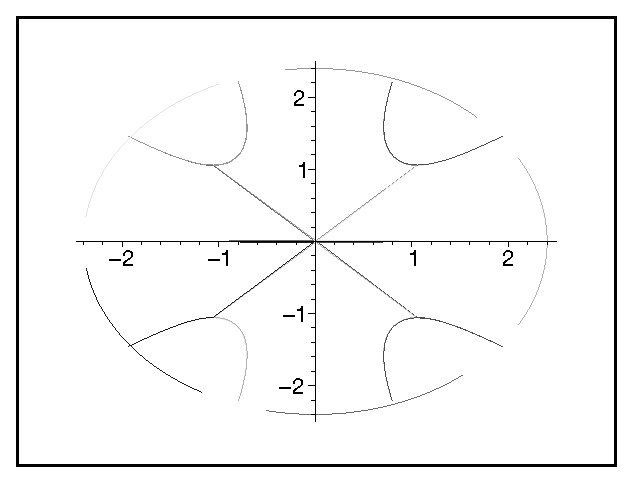
\includegraphics{rootbranch.eps}}
\caption{The branches of the \texttt{RootOf}$(z^5/5+z-w,index=k)$ function.
The circular arcs mark the extent of each branch.
Crossing the positive real axis is branch $k=1$,
and thereafter proceeding anticlockwise we have branches 2,3,4,5.
\label{fig:rootandbranch}}
\end{figure}

This example will not be analyzed further, but it has shown the potential in a branch
analysis for handling complicated inverse functions.

\section{Riemann surfaces}
A long standing treatment of multi-valued functions is based on Riemann surfaces.
Clearly it is important to see whether this treatment can be used instead of the one
presented here.
The question is one of fitness for computation, as opposed to conceptualization.
Thus it is true that Riemann surfaces give a very pictorial way of seeing
multi-valuedness~\cite{Trott:1997:VRS,RiemannW:1998}, but the question is whether
they can be used computationally.
This section makes a first attempt at such a computational interpretation.

Consider $f(z)=z^n$ and $\inversef{f}(z)=z^{1/n}$ as an example.
In the Riemann-surface treatment,
the function $\inversef{f}(z)$ continues to be regarded as a single valued function, but its argument
is now considered to lie on a multi-sheeted surface.
This is effectively how students in a first course on complex
numbers compute the $n$ values of $z^{1/n}$.
They are taught to start with the equivalence $z=re^{i\theta}=re^{i\theta+2\pi ik}$
and then mysteriously ordered to apply the rule $(e^{i\phi})^{1/n}=e^{i\phi/n}$
to the second form rather than the first.
Thus they are replacing $z$ with $z_k$, an equivalent point on the $k$th Riemann sheet,
and then computing $(z_k)^{1/n}$.

The difference between the approach of this paper, and the Riemann approach can be
summarized symbolically as $\inversef{f}_k(z)$ versus $\inversef{f}(z_k)$. We either distinguish
the function \textit{or} its argument.
Taking the point of view of a computer algebra system, we can notice that a complex number $z$
does not reveal its full significance until we know also the function for which it is an argument.
Advocates of Riemann surfaces have never, it seems, addressed issues of algebra on
Riemann surfaces.
Thus, when we write $\ln (uv)$, are $u$ and $v$ on the same sheet? That is, do we change
$u$ to $u_k$ and $v$ to $v_k$, where the $k$ is the same for each variable, or are we allowed to
write $v_l$? Further, what sheet is the product $uv$ on? Does the sheet of the product
depend upon the sheets of $u$ and $v$?
Moreover, if we write the expression $(z-1)^{1/2}+\ln z$, the Riemann surface for the
combined function is different from either of the component Riemann surfaces.
How do we label $z$?

We have to distinguish between a conceptual scheme and a computational scheme. Computer systems
are about computation. Often computation assists in conception, but computers must be able to
compute. Riemann surfaces are a beautiful conceptual scheme,
but at the moment they are not computational schemes.

\section{Conclusions}
Any attempt to change long ingrained mathematical habits must be regarded as largely a
Quixotic endeavour. The response of most readers to this paper will be
``Why should I change?" or more likely ``Damned if I'll change".
Most readers will defend the notation they use at present as being a perfectly
satisfactory notation for inverse functions.
Of course, most mathematicians would ardently defend XYZZY as being
ideal notation for inverse tangent, if that was what they were first taught.
But I won't be bitter; after all, I am human too.
Although students continue to be confused by the difference between $x^{-1}$ and $f^{-1}$,
some calculator companies have actually switched from labelling their keys asin and acos back to
labelling them $\sin^{-1}$ and $\cos^{-1}$ under pressure from their sales departments.

Until one has wrestled with a computer algebra system or with a non-elementary inverse function,
the urgency, or indeed the need, for new ways of looking at multi-valued functions is not apparent.
The current computer algebra systems are only just starting to adopt the
definitions given here.
Maple returns simplifications containing the function \texttt{csgn}, and
has to some extent trusted that users can be educated in this function.
The unwinding number
has been used in calculations, but is not yet returned explicitly to the user by any system.
It has been recommended for adoption in the Openmath standard~\cite{Corless:2000:AAS}.

For the average teacher of mathematics, the notation offered here holds out one immediate
advantage.
By teaching students the simple rule that $y=f(x)$ implies $x=\inversef{f}_k(y)$, where $k$
is arbitrary, we can hope to dispel some of the mystery of multi-valued functions. We already teach students
$y=x^2$ implies $x=\pm \sqrt y$, and we teach calculus students $dy/dx=1$ implies
$y = x+$ A CONSTANT. So solutions containing arbitrary elements are already part of
a student's education. By using branch indexing, we can bring all the elementary inverse
functions into this pattern.


\bibliographystyle {plain}
\bibliography{inversenote}

\end{document}
